\subsection{Phase II: Two-liquid-phase contact angle method}

The next method returns to the idea of water contact angles on metal surfaces. As described previously, water will spread completely on a nearly-flat metal surface surrounded by a gaseous environment. Instead of a gaseous environment, the water-metal system can be surrounded by another liquid. It has been observed that instead of wetting completely, a water droplet will only partially wet a metal when the surrounding environment is an immiscible liquid. This is called the two-liquid-phase contact angle method developed by Jacques Schultz.\cite{Schultz1977,Schultz1977a,Schultz1992} 


A full derivation of this method can be found in Appendix \ref{appendixB}. In order to calculate the dispersive component of \gamSV for a solid surface, the water \ca must be measured on a solid immersed in \nalk[s]. By interpreting Equation \ref{schultz2} as a classic linear function, $y = mx + b$:

\[
\underbracket{\gamma_{W}-\gamma_{H}+\gamma_{WH}\cos\theta_{W}}_{\text{\normalsize{$y$}}} =
\underbracket{2(\gamma_{S}^{D})^{1/2}}_{\text{\normalsize{$m$}}}  
\underbracket{[(\gamma_{W}^{D})^{1/2}-(\gamma_{H}^{D})^{1/2}] }_{\text{\normalsize{$x$}}} + 
\underbracket{I_{SW}^{P}}_{\text{\normalsize{$b$}}} 
\] 
$\gamma_{W}$, $\gamma_{H}$, and $\gamma_{WH}$ are known from consistently confirmed literature values,\cite{Chassin1986,Smitthipong2004,Takanashi2013,Nakamura2015} and are listed in Table \ref{knownsurften}. A data set of \textit{xy}-coordinates will be made by dropping water in an \nalk environment to determine $\gamma_{S}^{D}$ and $I_{SW}^{P} $. $\gamma_{S}^{D} $ will be calculated from the slope of the measured dataset. 

\begin{table}[h!]
	\centering
	\caption{Hydrocarbon surface tension and water-hydrocarbon interfacial energy}
	\begin{tabular} { |c||c|c|  } %\label{nalkSE}
		%	\hline
		%	\multicolumn{3}{|c|}{Hydrocarbon surface tension and water-hydrocarbon interfacial energy}\\
		\hline
		\textbf{\nalk[s]}	&\textbf{$\bm{\gamma_{H}}$ (mJ/m$\bm{^{2}}$)}	&\textbf{$\bm{\gamma_{WH}}$ (mJ/m$\bm{^{2}}$)}	\\
		\hline
		hexane		&18.4	&50.1 \\
		\hline
		octane		&21.7	&49.8 \\
		\hline
		decane		&23.8	&51.0 \\
		\hline
		hexadecane	&27.5	&51.3 \\
		\hline
	\end{tabular}
	\label{knownsurften}
\end{table}

%TODO: define London 

The polar component of the solid surface energy is determined using the same method described above,\cite{Schultz1977} but the bulk liquids now have both dispersive and polar components. This is also derived in Appendix \ref{appendixB}. These bulk liquids of chloroalkanes, nitroalkanes, aromatics, or alcohols are expected to establish a linear relationship between $I_{SW}^{P} $ and the square root of the polar component of surface tension from the bulk liquids. Schultz \etal suggests that this result allows all nondispersive interactions to be grouped together as a polar interaction, and they may be represented by the geometric mean of the polar component of the surface free energy of liquid and solid, as proposed by Owens and Wendt in Equation \ref{Isw}. This expression is verified experimentally, but there are no theoretical reasons why all nondispersive interactions should be represented by a geometric-mean expression.\cite{Fowkes1964}

\begin{equation}
\label{Isw}
	\begin{split}
	I_{SW}^{P} 							& = 2 (\gamma_{S}^{P}\gamma_{L}^{P})^{1/2} \\
	\rightarrow ~ \gamma_{S}^{P}	& = \frac{(I_{SW}^{P})^{2} }{4\gamma_{L}^{P}} 
	\end{split}
\end{equation}
The solid surface energy can then be determined from Equation \ref{gamS}:
\begin{equation}
\label{gamS}	\gamma_{S} = \gamma_{S}^{D} + \gamma_{S}^{P}	
\end{equation}

\begin{figure}[h]
	\centering
	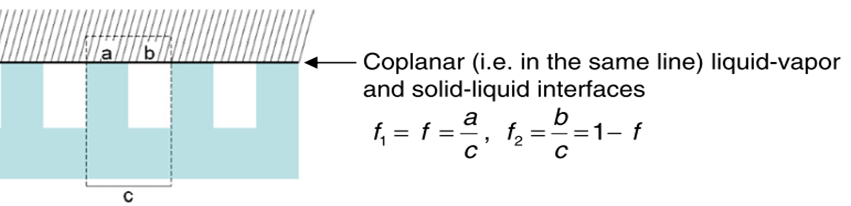
\includegraphics[width=0.7\linewidth]{cassie_coplanar}
	\caption{Schematic close up of three rough 2-D surfaces. Solid is blue/gray, air is white, liquid is the cross-hatched area above the surface. Liquid–vapor and solid–liquid interfaces of drop are denoted by the black line. A smooth-topped rough surface, which (for zero penetration of liquid) has coplanar solid–liquid and liquid–vapor interface (i.e. interfaces are in line with each other). This yields $ f_{1}=f $ and $ f_{2}=(1-f) $. Image source: \cite{Milne2012}}
	\label{fig:cassie_coplanar}
\end{figure}

Preliminary two-liquid-phase method experiments on muscovite mica showed quick and complete wetting of water on pristine mica surfaces cleaved in decane and hexadecane, contradictory to published results.\cite{Schultz1992} Clearly, more iterations of this experiment must be done to recreate this seminal paper's data, but this made me consider how a water droplet on a mirror-finished material of even greater surface energy (e.g. Fe and Fe alloys) would spread even faster than it had on a pristine mica surface. A \ca may not stabilize on a well-polished Galfenol sample even using this two-liquid-phase method, thus we must consider more options to create a measurable \ca that can extract Young's \ca. 

When mica samples were removed from the decane environment, they were wiped clean with lint-free wipes and further cleaned with acetone. When the samples were returned to the decane environment, a droplet wet the surface with an observable \ca. When this process was repeated in hexadecane, the observed \ca increased as observed in Schultz \etal This shows that even a rough surface can be measured for surface energy using the two-liquid-phase method. If this roughness is controlled by patterning the surface to a specific geometry, the same trend can be observed with the added benefit of a robust calculation of Young's contact angle by way of Equation \ref{cassie_coplanar}. 

Since Schultz published his seminal paper, his method has been used to measure very high surface energy materials ranging from ~50 mJ/m$^{2}$ to 487 mJ/m$^{2}$.\cite{Nakamura2015} However, many of these studies fail to consider the wetting modes of water on their solid surfaces in a bulk \nalk environment. Giljean \etal examines the dependence of contact angles on the roughness of high surface energy titanium surfaces using the two-liquid-phase method. They show that, depending on the cleaning technique used to remove surface contaminations, the contact angle will change more with a decrease in roughness. Sound arguments are made for the type of wetting regime (Wenzel, Cassie-Baxter, or somewhere in-between) encountered at each step of wetting. An issue occurs when the authors attempt to use the Cassie-Baxter equation to calculate the Young \ca. The Cassie-Baxter equation (Equation \ref{cassie_gen}), as defined in the original publication,\cite{Cassie1944} is designed for a general surface, where $f_1$ is the \textit{total} area of solid under the drop per unit projected area under the drop and $\theta_Y,1$ is the contact angle on a smooth surface of material 1. $f_2$ is defined similarly to $f_2$ where material 2 is air or some other medium. Many papers, as pointed out by Milne \etal,\cite{Milne2012} falsely use Equation \ref{cassie_coplanar} for randomly rough surfaces when this equation is for the special case of a coplanar liquid-vapor and solid-liquid interface, as illustrated in Figure \ref{fig:cassie_coplanar}. To use this simple equation, a surface would have to be patterned with rectangular pillars with a small enough spacing to prevent capillary forces from causing the liquid to penetrate the roughness. Keeping this in mind, I moved to the two-liquid-phase experiment originally performed on cleaved mica sheets. 
\begin{equation}
\label{cassie_gen}	
\cos\theta_{CB} = f_{1}\cos\theta_{Y} - f_{2}
\end{equation}
\begin{equation}
\label{cassie_coplanar}	
\cos\theta_{CB} = f\cos\theta_{Y} - (1-f)
\end{equation}

Considering all these factors, I postulate that by combining the two-liquid-phase method with a patterned surface of single-crystal Galfenol, the probe water droplet will not spread and a Young's \ca can be calculated for use in measuring the orientation-dependent surface energy of Galfenol. Single-crystal Galfenol samples were prepared at the DOE Ames Laboratory by the modified Bridgman technique at compositions of \fegacomp where $x=19,25$. These samples can be cut to obtain target orientations \hkl(100), \hkl(110), and \hkl(111) using electro-discharge machining. The isotropic surface created by single-crystal samples ensure that the triple-phase-line will maintain exactly the same $L_1-S$ interaction about the entire droplet perimeter. The patterned surfaces will be etched to have large enough pillars which retain as much surface orientation dependence on the contact angle as possible, as well as small enough gaps to allow for a Cassie-Baxter state in the $ L_1-L_2-S $ system. A Cassie-Baxter wetting mode would offer the greatest \ca of the three main wetting modes illustrated in Figure \ref{fig:young_cassie_wenzel}, and if a well patterned surface can be achieved similar to Figure \ref{fig:cassie_coplanar}, the Young \ca can be easily calculated from Equation \ref{cassie_coplanar}. 

Possible errors with this method will arise from non-atomically flat surfaces and pillars, imperfect Cassie-Baxter states caused by gravity or capillary forces drawing the probe liquid into the gaps between pillars, and oxide formation at the sample surface. However, such errors should be neglible given extensive polishing protocol, the immiscibility of water with \nalk[s], a controlled surface patterning, and a known cleaning procedure for rough metal surfaces. Therefore, I propose the assumption that our $ L_1-L_2-S $ system can be treated as the coplanar state depicted in Figure \ref{fig:cassie_coplanar} is reasonable. Concerning the displacement of \nalk[s] by water during the droplet depositing step, the wetting criteria has been proven by Schultz \etal\cite{Schultz1992,Giljean2011}. 

%This observable \ca is obviously a result of roughening the surface. , but because the trend of increasing \ca persists, I hypothesize that an induced roughness on isotropic metal surfaces could show increasing \ca[s] with increasing \nalk chain lengths. These induced roughnesses will be known, and using Wenzel\cite{Wenzel1936,Wenzel1949a} and Cassie\cite{Cassie1944} methods for calculating equilibrium \ca[s] and, resultantly, the orientation-dependent Galfenol surface energy. 
%TODO: CONTINUE HERE PLEASE. INSERT ASSUMPTIONS TO BE MADE AND THEN EXTEND TO ORIENTATION DEPENDENCE ON GALFENOL SINGLE CRYSTALS.

%\begin{figure}[h]
%	\centering
%	\begin{subfigure}[c]{0.47\textwidth}
%		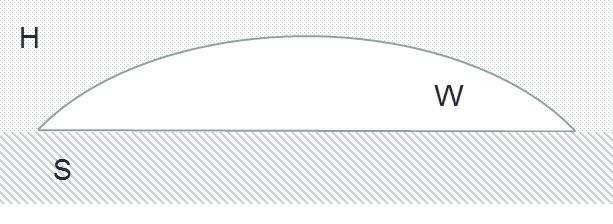
\includegraphics[width=\linewidth]{ideal-flat-two-liq}
%		\subcaption{~}
%		\label{fig:ideal-flat-two-liq}		
%	\end{subfigure}
%	\begin{subfigure}[c]{0.47\textwidth} 
%		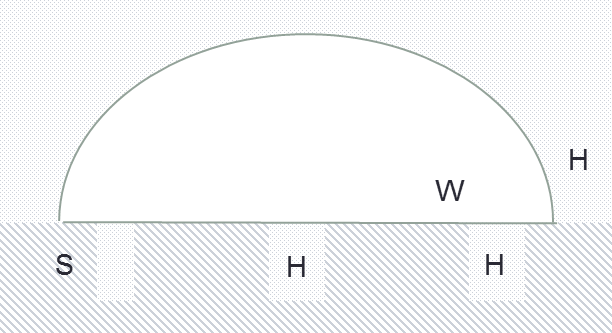
\includegraphics[width=\linewidth]{cassie-two-liq}
%		\subcaption{~}
%		\label{fig:cassie-two-liq}		
%	\end{subfigure}
%	\caption{(a) Ideally flat two-liquid-phase method (b) Cassie mode two-liquid-phase method }
%	\label{fig:goss_se_msrmnt}
%\end{figure}

\begin{figure}[h]
	\centering
	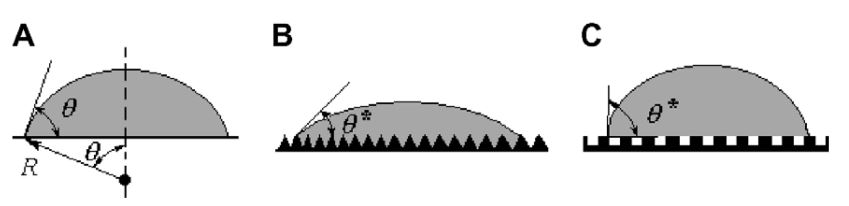
\includegraphics[width=\linewidth]{young_cassie_wenzel}
	\caption{Schemes of different wetting regimes. A – flat substrate; B – rough substrate, the Wenzel regime; C – rough substrate with air trapped under the drop, the Cassie–Baxter regime.\cite{Whyman2008}}
	\label{fig:young_cassie_wenzel}
\end{figure}

%The procedure for carrying out this study is as follows:
\subsubsection{Experimental plan}
%\renewcommand{\outlineii}{cenumerate}
%\begin{outline}[enumerate]
%\setlength{\itemindent}{0em}
\textbf{1)} For measuring the dispersive solid surface energy component, four different acrylic glass (Poly(methyl methacrylate), PMMA) boxes for hexane, octane, decane, and hexadecane environments will be used to contain the experiment. Acrylic has a high chemical compatibility with \nalk[s], and the transparent optical properties will not affect the contact angle pictures taken.\cite{Thermoscientific} Since most adhesives are stored in \nalk[s] (also commonly used as industrial strength degreasers), PMMA boxes must be chemically welded together by a solvent at room temperature to keep the liquid environment contained. The same boxes will be created for the other liquid mediums used to measure the polar solid surface energy component. \\
\textbf{2)} Single-crystal samples (\fegacomp where $x=19,25$) will be polished using SiC paper followed by 0.1 $\mu$m particle colloidal silica gel to achieve a mirror finish. EBSD or single-crystal XRD is used to find surface orientation. After the main sample surface orientation is discovered, the sample can be cut using wire cut electric discharge machining to obtain \hkl(001), \hkl(110), and \hkl(111) facets. Each sample is then polished again for EBSD measurement and surface energy measurement. As soon as polished samples have reached a mirror-finish, they will be immersed in the \nalk environment. \\ 
\textbf{3)} Samples will be mounted with the surface perpendicular to the dispensing needle and the two-liquid-phase method will be administered. This first experiment will attempt to measure a \ca on the polished Galfenol samples, but the probe water will likely spread over the surface very quickly to achieve complete wetting. Advancing and receding \ca[s] will be measured to find the contact angle hysteresis (CAH), as well as the drop volume of respective angles.  A group from the Max Planck Institute for Polymer Research has recently observed microscopic videos of water CAH on pillared polymer surfaces using laser scanning confocal microscopy.\cite{Butt2016,Schaffel2016} The UMD Department of Cell Biology and Molecular Genetics has two confocal microscopes that will be utilized to accurately measure the CAH of every Galfenol sample. By comparing this result to the CAH measured using the telescopic goniometer, we determine the necessity of confocal microscopy in future measurements. Another option for recording CAH is a high speed camera that to capture the wetting line spreading and receding. Coupled with the telescopic lens on the Kruss goniometer provided by UMD's Civil \& Environmental Engineering we can use a high speed CCD camera to capture such images. From the advancing and receding \ca[s], a proper averaging can be used to estimate the most stable contact angle, as seen in Equation \ref{avg_cah}.\cite{Andrieu1994} The most stable contact angle has also been measured by simply vibrating the system for ~15 s.\cite{Meiron2004} An averaging of advancing and receding \ca[s] is reasonable considering the practical advancing and receding \ca[s] are metastable states on opposite sides of a Gibbs energy vs. contact angle plot, seen in Figure \ref{fig:gibbs_ca}.
\begin{equation}
	\label{avg_cah}	
	\cos\theta_{ms} = (\cos\theta_{a} + \cos\theta_{r})/2 
\end{equation}
\begin{figure}
	\centering
	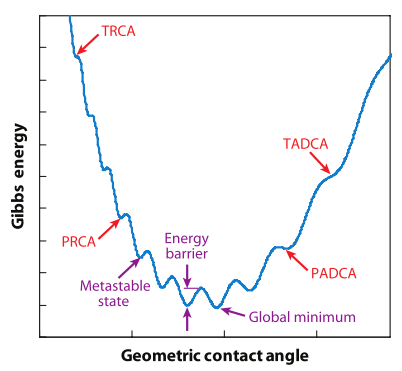
\includegraphics[width=\linewidth,trim={0 0 0 1cm}]{gibbs_ca}
	\caption{The curve of Gibbs energy versus geometric contact angle for a two-dimensional drop on a heterogeneous solid surface. Each minimum represents a metastable equilibrium state. The lowest of all minima indicates the most stable state. In between every pair of equilibrium states there exists an energy barrier. Abbreviations used: PADCA, practical advancing contact angle; PRCA, practical receding contact angle; TADCA, theoretical advancing contact angle; TRCA, theoretical receding contact angle.\cite{Marmur2009b}}
	\label{fig:gibbs_ca}
\end{figure}
The drop volumes of advancing and receding \ca[s] will give us a range of volumes for static \ca measurements on the same surfaces, which are also expected to totally wet our flat surfaces, but will be measured to validate that assumption.\\
\textbf{4)} I will  work with UMD's FabLab to determine the best protocol for creating a patterned surface on Fe-Ga samples. Patterning will occur on the mirror-finish samples made in Step 2 to ensure the flattest possible pillars. With well patterned surfaces, I will execute the same two-liquid-phase method procedure described in Step 3. I expect much greater contact angles for every surface based on the controlled roughness, and I also expect dramatic differences in the calculated solid surface energies for the \hkl(100), \hkl(110), and \hkl(111) Fe-Ga surfaces using Equation \ref{gamS}. \\
\textbf{5)} These surface energy values should be similar to the $\alpha$-iron DFT calculations of $\gamma_{100}$ = 2.6660 J/m$^2$, $\gamma_{110}$ = 2.0535 J/m$^2$, and $\gamma_{111}$ = 2.5271 J/m$^2$.\cite{Wang2000} While testing single-crystal samples of two different compositions (\fegacomp where $x=19,25$), it is unclear how the surface energy of Fe-Ga will change with composition. I have asked our collaborator, Dr. Ruqian Wu, to use computer simulations to try and find such a change in surface energy with composition, which I will compare with upon experimentally determining these values. 
%Pattern surfaces with transparency paper $\gtrsim$40 $\mu$m since this is the lower limit of transparency paper. 



%	\2 The assumption of this patterned surface is that the Cassie-Baxter or Wenzel contact angle is the most stable contact angle, and the Young contact angle can be approximated using the Cassie-Baxter and Wenzel equations. This contact angle will be suitable for the of metal surface energy that will be calculated from Equation \ref{schultz2}.
%		\3 There seems to be controversy in literature on whether the equilibrium contact angle calculated in Cassie and Wenzel equations can be used as the Young \ca.\cite{Attension2015,Marmur2009b,Bracco2013}
%		\3 The Cassie-Baxter contact angle is an equilibrium contact angle as proven by Johnson and Dettre using thermodynamic principles.\cite{Johnson1964}
%		\3 The most stable contact angle on a rough surface is either the Wenzel or Cassie angle, IF the size of the drop is two to three orders of magnitude larger than the typical scale of roughness.\cite{Meiron2004} %TODO: read the paper cited, about sufficient drop size vs. roughness
%	\2 Preliminary two-liquid-phase method experiments on muscovite mica showed quick and complete wetting of water on pristine mica surfaces cleaved in decane and hexadecane, contradictory to published results.\cite{Schultz1992} When mica samples were removed from the decane environment, they were wiped clean with KimWipes and further cleaned with acetone. When the samples were returned to the decane environment, a droplet wet the surface with an observable \ca. When this process was repeated in hexadecane, the observed \ca increased as observed in Schultz et al.\cite{Schultz1992} 
%	
%	This observable \ca is a result of roughening the surface, but because the trend of increasing \ca persists, I hypothesize that an induced roughness on isotropic metal surfaces could show increasing \ca[s] with increasing \nalk chain lengths. These induced roughnesses will be known, and using Wenzel\cite{Wenzel1936,Wenzel1949a} and Cassie\cite{Cassie1944} methods for calculating equilibrium \ca[s] and, resultantly, the orientation-dependent Galfenol surface energy. 
%		
%	\2 Per conversation with Dave Shahin, an experienced student in patterning surfaces, an array of roughnesses can be made on a single sample to test roughness effects on surface energy measurements of single crystal Galfenol and Alfenol. 
%		\3 There is a criteria for determining if the calculated contact angle on a rough surface is in Wenzel and Cassie-Baxter modes.\cite[p. 53]{Milne2012}
%	
%\1 Redo two-liquid-phase experiment for patterned surface
%	\2 Calculate the Cassie and Wenzel mode equilibrium CA
%		\3 Expecting Cassie mode because the patterned channels will ideally be completely filled with hydrocarbon/\nalk liquid, thus \underline{repelling} the water droplet on the surface. This is due to the immiscibility of polar (distilled water) and non-polar (\nalk) solvents. 
%	\2 \textbf{Is there a difference from one patterned orientation to another?} This will show if the patterning (induced roughness) will have a large impact on the CA and, as a result, \underline{Surface Energy}. 
%		\3 If we have a defined roughness for {100}, {110}, and {111} samples, and the apparent \ca[s] do not change with orientation, the geometry of the roughness dictates the \ca. 
%		\3 If the \ca[s] do change with orientation, the surface orientation determines the \ca, and surface energy can be confidently measured.
%\end{outline}

Pending the success of this proposed research, our group will incorporate these experimentally determined orientation-dependent surface energies into to our AGG model to elucidate the driving forces of grain growth methods in Galfenol. We would like to expand this experiment to single-crystal Alfenol samples as well as many other pure and alloyed metals. Metal surface energies are extremely elusive values due to their complexities and lack of consistent experimental confirmation. My goal is that this work will contribute to the vast body of work on experimental wetting dynamics and surface energy determination for the benefit research in the near future and push the boundaries of understanding.


%\subsection{Timeline}
%What follows in Table [  ] is a projected timeline for completion of the proposed research, leading to a defense and graduation in the Winter of 2017. 


%\subsection{Induced roughness for Wenzel and Cassie modes}

%\subsection{DFT measurements from collaborator}
%\subsubsection{Cassie-Baxter or Wenzel mode}
%\textbf{Can Dr. Ruqian Wu simulate a sessile drop in a two-liquid-phase experiment on a patterned surface?} This can tell us if we can expect Cassie of Wenzel mode of water drop in hydrocarbon/\nalk environment. 
%
%\subsubsection{Two compositions of single crystal Galfenol}
%Dr. Wu has assigned a student to working on a difference in \fegacomp surface energy where $x =$ 19 and 25.